\chapter{Models and Simulations}

A simulation is intended to imitate in many cases, a real-world process or system, that may be too difficult or costly to analyze directly. Before any such simulation can begin, a model of the system studied must be constructed. Models capture the characteristics and behaviours of the system they represent and in general, a model should be as simple as possible (since resources are limited) while still explaining experimental observations and making predictions with a given degree of accuracy. The simulation is the implementation of the model and can be executed on a computer to produce data for testing, analysis, and visual presentation.

In our simplified model of a biological tissue, the relatively ordered and periodic nature of cells in most simple tissues is captured as a series of repeating \textit{unit cells}. These unit cells are the building blocks of the heterogeneous 1D and 2D models. Each unit cell is characterized by a cellular domain, separated from an extracellular domain by a semi-permeable membrane. Both domains are isotropic everywhere except at the boundaries. Regarding the boundaries, there exists two kinds in our models. The first kind is a totally-reflecting boundary; it forms the absolute boundary of the model system and represents an insurmountable physical barrier. The second kind is a semi-permeable non-active/passive boundary and represents the selectively permeable nature of the plasma membrane. In a real biological plasma membrane, the integral membrane proteins may facilitate active or passive transport. More specifically, in the simple cell model, the semi-permeable membranes behave in a passive transport manner and this is implemented as a transition probability, a concept explained in Section \ref{sec:intro-diffusion}.

So what is being simulated? 
Currently, there is no net force on the particles (no directed motion) and the particles are non-interacting.

For all 1D and 2D models, both Monte Carlo and master equation approaches were used to simulate the diffusion of particles on a lattice.

Step size is fixed and equal in all directions

Particle motion occurs along a line in the 1D simulation and two orthogonal directions in the 2D simulation.

\section{1-Dimensional Systems}
In 1D, homogenous and heterogeneous simple cell systems were simulated using Monte Carlo (MC) and master equation approaches. 

\subsection{Homogenous System}


*include figure of homogenous model*

\subsection{Heterogeneous System}


*include figure of heterogeneous model*

\section{2-Dimensional System}

\begin{figure}[h]
	\centering
	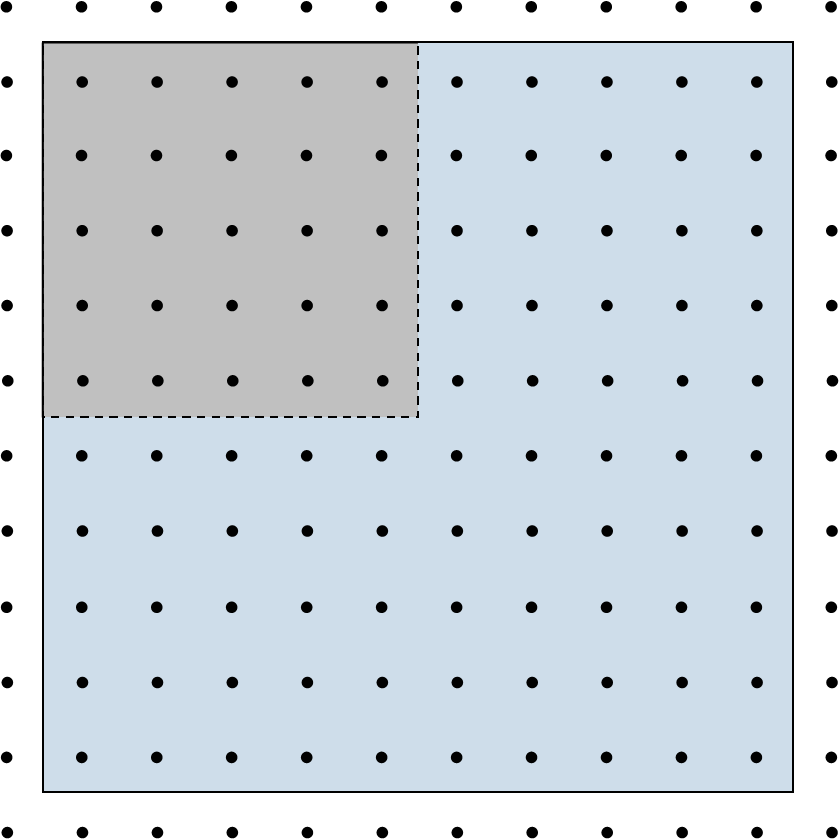
\includegraphics[width=0.5\linewidth]{2d_unit_cell_1.png}
	\caption{2D lattice unit cell with cellular and extracellular regions. Dashed lines indicate semi-permeable barrier.}
	\label{fig:2d_unit_cell_1.png}
\end{figure}
*include figure of heterogeneous model*